 
\begin{figure}[h]
\centering
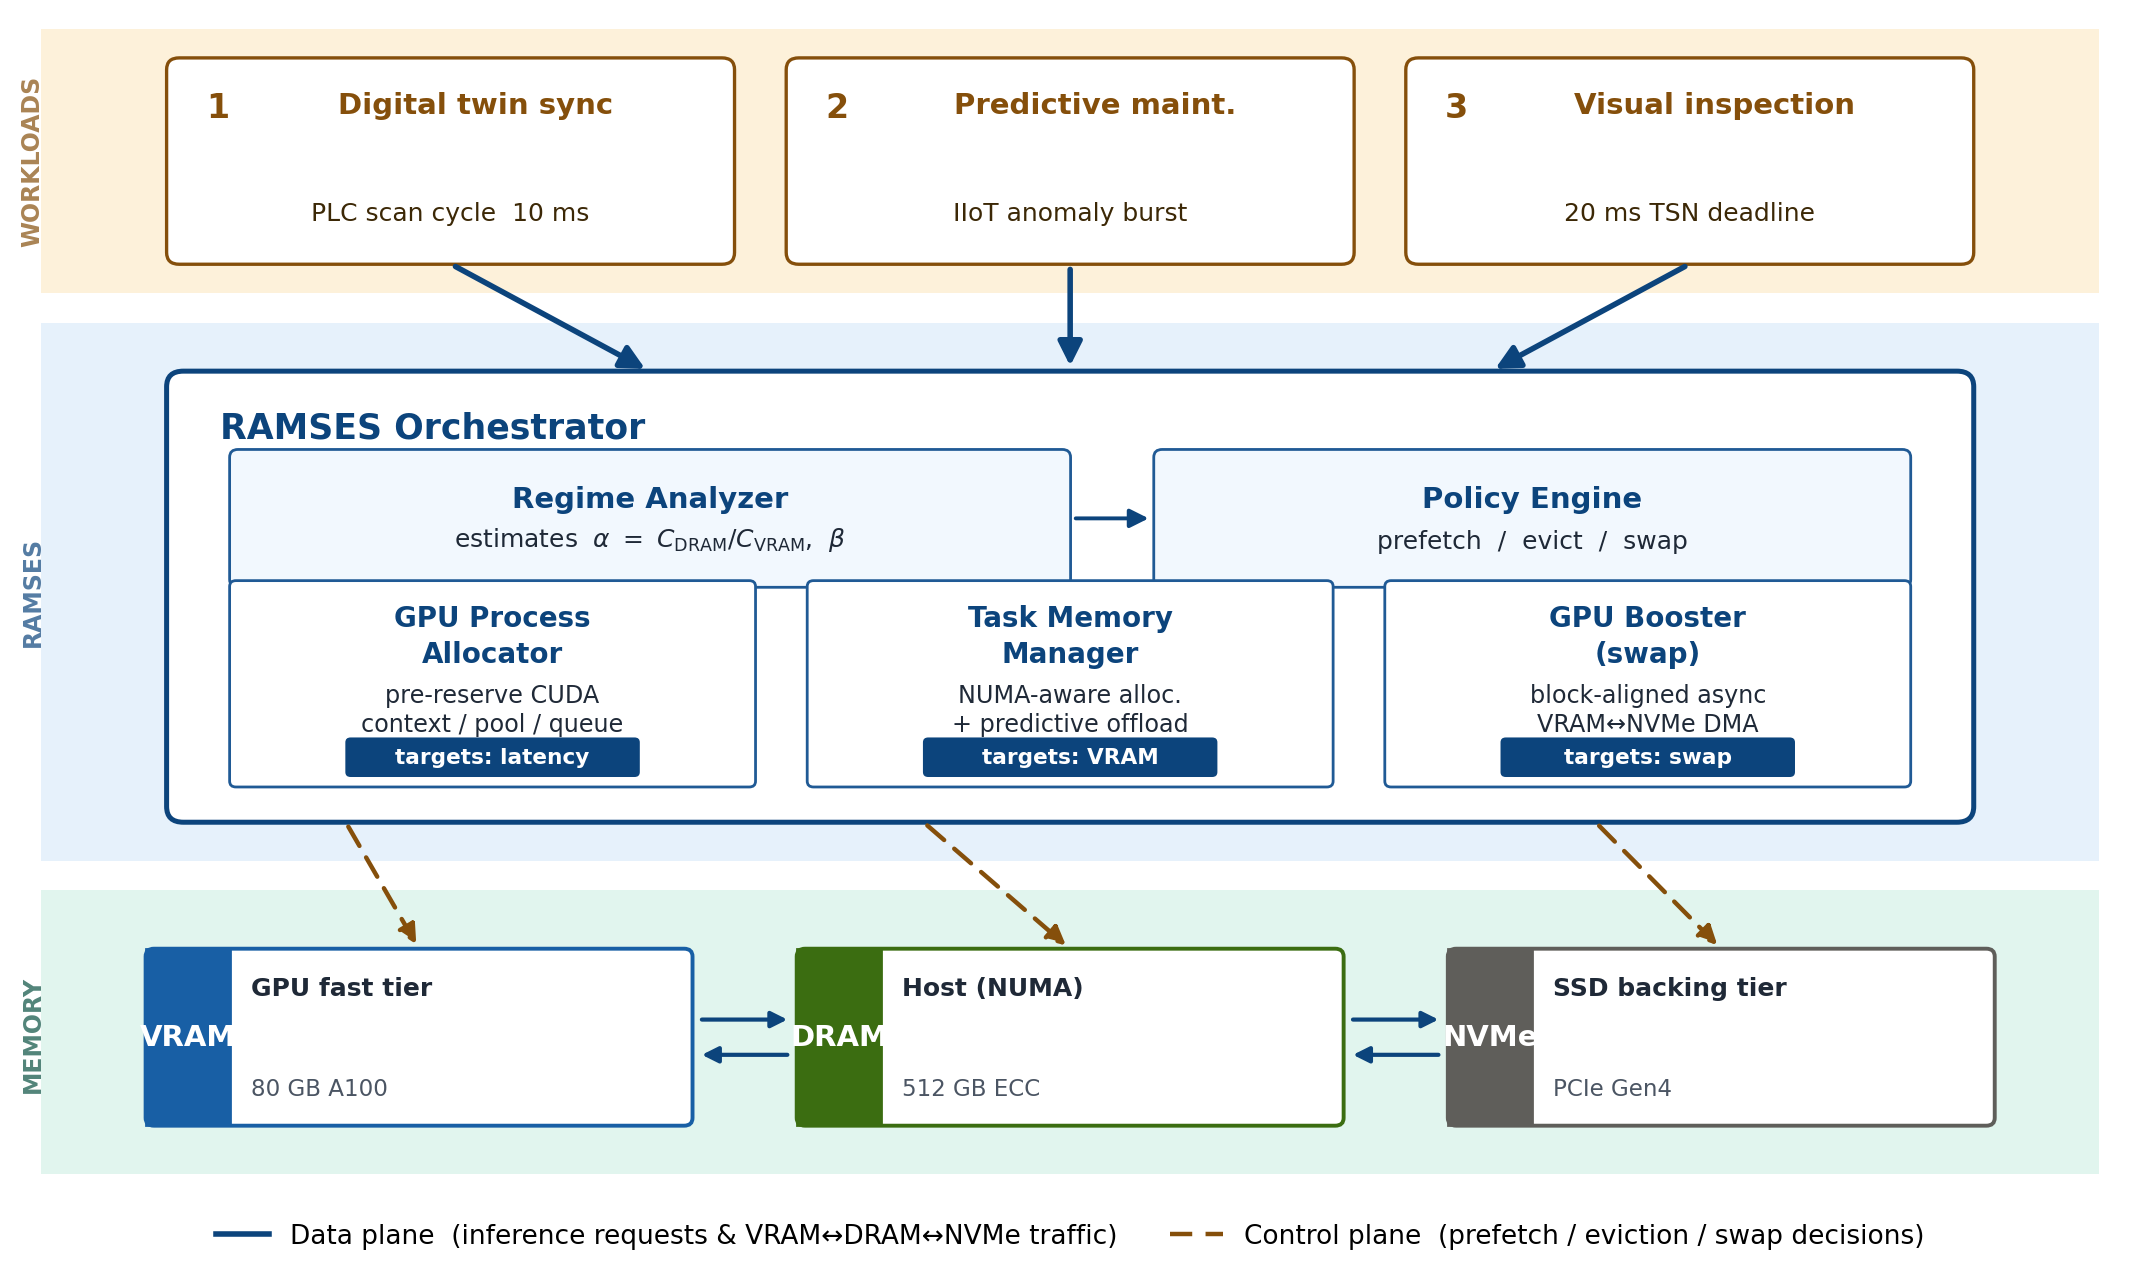
\includegraphics[width=0.95\linewidth]{figures/rameses_design.png}
\caption{Industrial hierarchical memory architecture of RAMSES
for laboratory workloads motivated by industrial analytics.
The data plane (solid arrows) coordinates GPU VRAM, host DRAM,
and NVMe for three industrial workloads:
(1) digital twin state synchronization aligned with PLC scan cycles,
(2) predictive maintenance triggered by anomaly bursts from IIoT sensors,
and (3) real-time visual inspection under bounded inference deadlines.
The control plane (dashed arrows) includes a Regime Analyzer
estimating $(\alpha,\beta)$ and a Policy Engine enforcing tier-aware
placement, prefetch, and swap decisions.
Three modules handle the actual orchestration:
the \emph{GPU Process Allocator} pre-reserves CUDA context to remove
context-conflict stalls,
the \emph{Task Memory Manager} performs NUMA-aware allocation with
predictive DRAM offloading,
and the \emph{GPU Booster} drives block-aligned asynchronous VRAM--NVMe
swap.
This architecture explicitly links intra-node memory orchestration
to industrial control loops, TSN time windows, and SLA-constrained
operation.}
\label{fig:rameses_architecture}
\end{figure}

\section{RAMSES: Architecture and Key Components}\label{sec:mball}
\footnotetext[1]{The anonymized synthetic-trace generator is included with the review artifact. Runtime source and baseline ports require a separate archival release before resubmission.}

LLM inference relies on tight cooperation across a heterogeneous set of resources: GPUs, VRAM, DRAM, NVMe, and Central Processing Units (CPUs). Existing serving stacks and runtimes do not handle resource contention as a first-class concern, which is why we keep seeing the same failure modes: Compute Unified Device Architecture (CUDA) out-of-memory (OOM) errors, context-switch stalls, and memory-mapping overhead. Earlier attempts to plug these gaps include GPU--CPU offloading~\cite{xu2025ellm}, speculative offloading~\cite{zhuge2025specoffload}, and cache-centric management~\cite{jiang2024neo}. Useful as those are, most stop at single-tier transfers (typically VRAM--CPU) or address only narrow scenarios such as key-value (KV) cache management.

We propose \textbf{RAMSES} as a way past these limits. The design borrows the OS notion of memory ballooning and applies it to LLM serving. What separates RAMSES from prior work is that it manages the whole VRAM--DRAM--NVMe hierarchy together: GPU context conflicts, NUMA-induced latency, and inefficient swapping are addressed in the same control loop instead of patched independently. RAMSES also reallocates GPU and system memory on the fly, while staying lightweight enough to avoid the deployment burden of full distributed-processing frameworks. Three modules sit at the core of the design---the \textbf{GPU Process Allocator}, the \textbf{Task Memory Manager}, and the \textbf{GPU Booster with swap support}---and they are illustrated in Fig.~\ref{fig:rameses_architecture}.

\subsection{GPU Process Allocator}
In multi-model serving, two bottlenecks dominate: \textbf{GPU context loading conflicts} and \textbf{VRAM interference}. CUDA drivers do context initialization and memory mapping with \textit{lazy binding}, which is fine for a single workload but becomes painful under concurrent execution---startup delays grow, and they show up directly in user-facing latency. NEO \cite{jiang2024neo} addresses cache management but leaves the GPU-level context conflict question open.
The \textbf{GPU Process Allocator} is our answer to this. Rather than waiting for runtime to resolve these conflicts, it reserves GPU execution resources up front: context IDs, memory pools, and kernel queues are pre-assigned. It also keeps memory segments separated across models, which keeps cache pollution down, and it co-schedules I/O-intensive and compute-intensive models so the GPU is not idle waiting on either side.

In practice, the allocator runs three policies.
\textbf{Pre-defined execution slot reservation} hands each model a context ID, memory pool, and kernel queue ahead of time, so CUDA initialization no longer happens on the critical path.
\textbf{Context separation with fixed memory pools} assigns models to separate configured regions; the finite experiments show lower fragmentation and cross-model cache interference.
\textbf{Priority-based scheduling} orders execution between I/O-bound and compute-bound models so neither stalls the other and idle GPU cycles shrink.
The result is a small extension of process pinning that helps preserve \textbf{Quality of Service (QoS) stability} and gives more \textbf{predictable latency} when several models share one GPU \cite{stojkovic2025dynamollm}. Algorithm~\ref{alg:gpa_en} summarizes the end-to-end pre-reservation and dispatch flow.

% -- Pseudocode for GPU Process Allocator (English) --
\begin{algorithm}[t]
\caption{GPU Process Allocator Pseudocode}
\label{alg:gpa_en}
\begin{algorithmic}[1]
\Require Set of models $\mathcal{M}$, GPU resource pool $\mathcal{R}$
\State Initialize free context IDs, memory pools, and kernel queues
\For{each model $m \in \mathcal{M}$}
  \State Reserve a context ID, memory pool, and kernel queue for $m$
  \State Assign a priority based on whether $m$ is I/O-bound or compute-bound
\EndFor
\While{tasks remain}
  \State Dequeue the next task $t$ based on priority
  \State Launch $t$ on its reserved context
  \If{$t$ finishes}
    \State Return its resources to $\mathcal{R}$
  \EndIf
\EndWhile
\end{algorithmic}
\end{algorithm}


\subsection{Task Memory Manager}
Memory usage during LLM inference shifts back and forth between DRAM and VRAM as input and generation lengths change. eLLM \cite{xu2025ellm} responded to this by extending the CPU buffer; PIE \cite{xu2024pie} took a speculative-swap approach. Neither, though, paid attention to NUMA-induced latency or to optimization within DRAM itself.

Our \textbf{Task Memory Manager} closes that gap. It pairs task-level memory control with NUMA-aware policies: by aligning processes with the right memory nodes, remote-access delay is reduced, and a jemalloc-based custom heap separates small objects from large tensors so that fragmentation stays manageable \cite{hunter2021hugepage,yang2023numalloc}. On top of this, the module looks ahead: tensors with low expected access probability are offloaded preemptively, and a small predictive model of memory pressure feeds anticipatory decisions \cite{korthikanti2023reducing}.
We model memory access latency as
\[
T_{access} = T_{local} + \gamma \cdot T_{remote},
\]
where $\gamma$ is the penalty factor from a remote NUMA access.
Bad allocation policy here cascades---excessive \textit{page reclaim}, \textit{mmap} failures, unnecessary \textit{buffer eviction}. Existing fixes mostly fall back to reactive GPU offloading or memory compression once VRAM gets tight; they leave DRAM behavior and NUMA locality on the table.

The Task Memory Manager has four pieces.
\textbf{NUMA-aware memory mapping} pins process and thread data to local NUMA nodes through system calls such as \texttt{mbind()} and \texttt{numa\_alloc\_onnode()} so that remote-memory traffic is minimized.
\textbf{jemalloc-based heap optimization} tunes pool size, allocation granularity, and cache-aware placement, with small objects kept apart from large tensors.
\textbf{Task-level redistribution} watches per-request memory consumption and offloads non-critical tensors to DRAM before VRAM saturates.
\textbf{A lightweight memory pressure prediction model} reads live utilization and I/O queue depth to predict shortages and trigger mitigation early.
Together, these free up VRAM and---a point worth highlighting---make DRAM--VRAM use more efficient as a unit, with less fragmentation and fewer \textit{page reclaim} events. RAMSES is therefore able to keep memory provisioning stable and access latency low even when several models and processes contend for the same node. Algorithm~\ref{alg:tmm_en} states the full NUMA-aware allocation and predictive offloading procedure.

% -- Pseudocode for Task Memory Manager (English) --
\begin{algorithm}[t]
\caption{Task Memory Manager Pseudocode}
\label{alg:tmm_en}
\begin{algorithmic}[1]
\Require Execution graph $G$, memory threshold $\tau$
\State Bind threads to local NUMA nodes using OS calls (e.g., \texttt{numa\_alloc\_onnode})
\State Initialize separate jemalloc heaps for small objects and large tensors
\For{each incoming request $r$}
  \State Monitor VRAM usage and fragmentation
  \If{usage $> \tau$}
    \State Identify tensors in $G$ with low immediate reuse probability
    \State Offload these tensors to DRAM/NVMe
  \EndIf
  \State Use a lightweight predictor to anticipate memory pressure based on current utilization and I/O depth
  \State Pre-allocate VRAM/DRAM resources for the next request
\EndFor
\end{algorithmic}
\end{algorithm}


\begin{table*}[t]
\centering
\renewcommand{\arraystretch}{1.0}
\caption{Comparison of RAMSES with existing baselines. Each row identifies a baseline serving stack, its key optimization technique (\emph{Key Features}), the reason it was selected for evaluation (\emph{Rationale}), and which RAMSES module addresses the corresponding bottleneck (\emph{Targeted by RAMSES}). Citations refer to the baseline systems.}
\label{tab:baseline_comparison}
\begin{tabular}{|p{3.8cm}|p{3cm}|p{3.5cm}|p{3.5cm}|}
\hline
\textbf{Method} & \textbf{Key Features} & \textbf{Rationale} & \textbf{Targeted by RAMSES} \\
\hline
Default (PyTorch) & No optimization & Ground truth reference & Overall performance gain \\
\hline
FlexGen~\cite{sheng2023flexgen} (ICML'23) & CPU offloading & VRAM expansion via offload & GPU Booster (swap) \\
\hline
SwapAdvisor~\cite{swapAdvisor2020} (ASPLOS'20) & GPU--CPU swap & Canonical swap optimization & Task Memory Manager \\
\hline
NEO~\cite{jiang2024neo} (MLSys'25) & KV cache offload + sched. & Recent tier utilization & Hierarchical (full) tier use \\
\hline
SpecOffload~\cite{zhuge2025specoffload} (arXiv'25) & Cross-tier swap min. & Latest transfer optimization & NVMe--VRAM transfer path \\
\hline
vLLM~\cite{kwon2023pagedattention} (SOSP'23) & KV cache + streaming & SOTA inference optimization & End-to-end latency \\
\hline
\end{tabular}
\vspace{-12pt}
\end{table*}

\subsection{GPU Booster with Swap Support}
VRAM capacity remains one of the hardest constraints in serving large models. FlexGen \cite{sheng2023flexgen} and SwapAdvisor \cite{swapAdvisor2020} support GPU--CPU swapping, but neither is tuned to GPU memory hierarchies in particular.

The \textbf{GPU Booster with swap support} module addresses this. It walks the execution graph to spot inactive tensors and overlaps their movement with computation by way of direct Peripheral Component Interconnect express (PCIe) Direct Memory Access (DMA) and asynchronous I/O. Swap units are aligned to 4MB boundaries to avoid wasted transfers. With these mechanisms in place, RAMSES served models up to 17B parameters on GPUs with less than 80GB of VRAM, and we did not observe instability during the experiments.

Conventional offloading typically pays a noticeable transfer cost, and OS-level swapping is unaware of GPU memory semantics, which limits how well it can do.
The swapping mechanism here is GPU-aware. It performs \textbf{selective tensor offloading}, using execution-graph analysis to flag tensors that are not immediately needed---inactive attention key/value caches, intermediate checkpoints---as swap candidates. To reduce the cost further, the system runs an \textbf{optimized I/O path}: VRAM-to-NVMe transfers go through direct PCIe DMA, with asynchronous I/O queues so that transfer and compute proceed in parallel. \textbf{Priority-aware and block-aligned swapping} aligns swap blocks to 4MB units; the scheduler weighs both tensor size and reuse frequency. When a cache miss does happen, partial reloads keep transfer volume small.

The combined effect is that RAMSES can keep \textbf{17B-parameter models} serving on memory-constrained GPUs while holding swap-induced latency to a minimum \cite{kwon2023pagedattention}. Algorithm~\ref{alg:gbooster_en} pins down the swap-aware asynchronous control flow, including the selective tensor identification, block-aligned DMA transfer, and partial reload after a cache miss.
\begin{algorithm}[t]
\caption{GPU Booster with Swap Support Pseudocode}
\label{alg:gbooster_en}
\begin{algorithmic}[1]
\Require Execution graph $G$
\For{each tensor $t$ in $G$}
  \If{$t$ is not required in upcoming compute steps}
    \State Align $t$ to 4MB boundaries
    \State Initiate asynchronous DMA transfer of $t$ to NVMe storage
    \State Mark $t$ as swapped out
  \EndIf
\EndFor
\While{serving requests}
  \If{the next computation step reaches a swapped-out tensor $t$}
    \State Partially reload $t$ via asynchronous DMA from NVMe
    \State Resume computation once the needed portion of $t$ has been fetched
  \EndIf
\EndWhile
\end{algorithmic}
\end{algorithm}

%----------------------------------------------------------------

\begin{figure}[t]
\centering
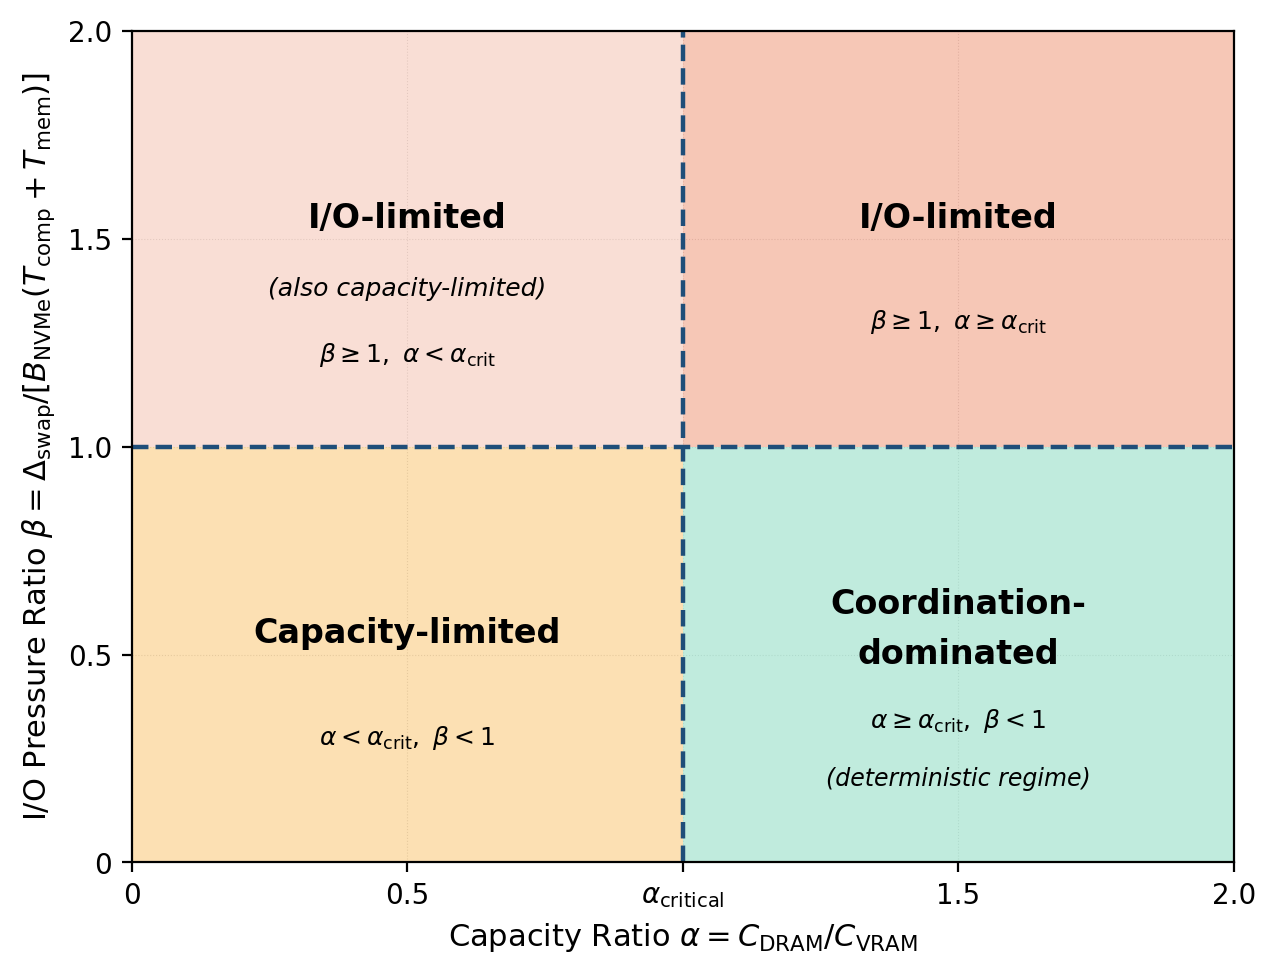
\includegraphics[width=0.95\linewidth]{figures/phase_diagram.png}
\caption{Schematic operating map for the measured pressure ratios. Here $\alpha=D/C_f$ denotes capacity pressure and $\beta$ is the ratio of non-overlapped transfer time to compute, memory, and synchronization time. The dashed lines are operational classification thresholds, not feasibility, determinism, or stability guarantees; measured operating points and prediction residuals accompany the artifact.}
\label{fig:phase_diagram}
\end{figure}

\subsection{Overlap-Aware Operating Model}\label{sec:theory}

We use the following model as an engineering classification tool, not as a
real-time guarantee.  Let $D(t)$ be the bytes resident or demanded by a step,
$C_f=C_{\mathrm{VRAM}}+C_{\mathrm{DRAM}}$ the usable fast-tier capacity,
$V_{\uparrow}(t)$ and $V_{\downarrow}(t)$ the measured read and write transfer
volumes, $h(t)$ the prefetch-hit fraction, and $q(t)$ the measured storage
queueing delay.  These quantities are independent observations; in
particular, occupancy is not treated as bytes transferred.  The capacity
pressure is
\begin{equation}\label{eq:alpha_def}
 \alpha(t)=D(t)/C_f,
\end{equation}
and the transfer pressure is
\begin{equation}\label{eq:beta_def}
 \beta(t)=\frac{L_0+q(t)+V_{\uparrow}(t)/B_{\uparrow}
 +V_{\downarrow}(t)/B_{\downarrow}}
 {T_{\mathrm{comp}}(t)+T_{\mathrm{mem}}(t)+T_{\mathrm{sync}}(t)}.
\end{equation}
Here $L_0$ is fixed request/setup latency and $B_{\uparrow}$ and
$B_{\downarrow}$ are effective, direction-specific bandwidths measured with
the same block size and queue depth as the experiment.  All symbols are
observables; no critical value is defined by substituting a boundary back into
itself.

Asynchronous transfer overlaps computation.  Accordingly, predicted service
time is
\begin{IEEEeqnarray}{rCl}\label{eq:latency_total}
\widehat T_{\mathrm{total}} &=& T_{\mathrm{{sync}}}+T_{\mathrm{mem}}
 +\max\{T_{\mathrm{comp}},(1-h)T_{\mathrm{xfer}}\},\\
T_{\mathrm{xfer}}&=&L_0+q+V_{\uparrow}/B_{\uparrow}+V_{\downarrow}/B_{\downarrow}.
\end{IEEEeqnarray}
The max operator prevents double counting overlapped DMA and compute.  Block
rounding is included in the measured volumes.  We call observations with
$\alpha>1$ capacity-pressured and observations with $\beta\geq1$ transfer-
pressured; the remaining points are coordination-sensitive.  These are
operational labels, not theorems.  They neither imply zero swapping nor a
worst-case bound.  Fig.~\ref{fig:phase_diagram} is therefore a schematic guide;
measured points and prediction residuals are reported with the evaluation
artifact.

\subsection{Online Policy and Complexity}\label{sec:controller}
Every 200~ms the analyzer reads allocated bytes, transfer counters, queue
depth, effective bandwidth, and exponentially weighted compute, memory, and
synchronization times.  It computes Eqs.~\eqref{eq:alpha_def}--\eqref{eq:beta_def}
in constant time.  To avoid oscillation, a state change requires three
consecutive samples beyond a 5\% hysteresis band.  In the capacity-pressured
state the policy rejects admissions that exceed the configured memory reserve
and evicts the lowest predicted-reuse tensors.  In the transfer-pressured state
it stops speculative eviction, reduces prefetch depth, and prioritizes reads.
In the coordination-sensitive state it enables asynchronous prefetch and
NUMA-local placement.  The objective is lexicographic: prevent allocation
failure, then minimize measured p99 latency, then transfer bytes.

The reuse score is an exponentially weighted count of accesses over the last
32 graph steps; it has no learned parameters or offline training.  Candidate
maintenance costs $O(\log n)$ per tensor access for a heap of $n$ evictable
tensors; sampling, regime classification, and a policy decision are $O(1)$,
and metadata occupies $O(n)$.  A policy-off ablation retains all three data-
plane modules but fixes prefetch depth and disables state switching, separating
the controller from its mechanisms.  The reported 1.68~ms is mean controller
work per serving request and is not compatible with a 2~ms end-to-end claim;
we therefore make no such claim.

\subsection{Scope of Timing and Safety Claims}
The measured latency distributions are QoS observations for non-safety AI
serving.  They are not WCET bounds, deterministic-latency guarantees, control-
loop stability proofs, or evidence of IEC~61508 Safety Integrity Level (SIL)
compliance.  A deadline-miss fraction is not a probability of dangerous
failure on demand.  Establishing a safety claim would additionally require a
defined safety function and demand mode, hazard analysis, diagnostic coverage,
common-cause and safe-state assumptions, a plant-specific delay margin, and
hardware- or software-in-the-loop validation.  RAMSES must therefore be kept
outside a safety function unless independently qualified by the integrator.

\subsection{Ablation Analysis}
The three modules of RAMSES contribute on their own, but they also reinforce each other when combined. To show this, we ran an \textbf{ablation study} over four configurations: full RAMSES, RAMSES without the GPU Process Allocator, without the Task Memory Manager, and without the GPU Booster. Table~\ref{tab:ablation} summarizes the outcome---every ablation degrades performance, and the breakdown matches the design intent of each module. Removing the \textbf{GPU Process Allocator}, in particular, has the largest impact on inference latency (35.0\% $\rightarrow$ 20.5\%, a 14.5~percentage-point drop), consistent with its role of pre-resolving CUDA context conflicts on the critical path. Removing the \textbf{Task Memory Manager} has the largest impact on VRAM reduction (15.0\% $\rightarrow$ 5.0\%, a 10.0~percentage-point drop), consistent with its NUMA-aware allocation and predictive DRAM offloading. Disabling the \textbf{GPU Booster} produces an intermediate degradation across both latency and VRAM, consistent with its swap-aware role between VRAM and NVMe. The pattern lines up cleanly with the design intent: each of the three modules dominates the metric it was built to target~\cite{korthikanti2023reducing}.

\begin{table}[h]
\centering
\renewcommand{\arraystretch}{1.1}
\caption{Ablation study results: Impact of disabling RAMSES modules}
\label{tab:ablation}
\begin{tabular}{|l|c|c|c|}
\hline
\textbf{Configuration} &
\makecell{\textbf{Load Time} \\ \textbf{Reduction}} &
\makecell{\textbf{Latency} \\ \textbf{Reduction}} &
\makecell{\textbf{VRAM} \\ \textbf{Reduction}} \\
\hline
Full RAMSES             & 58.7$\pm$1.8\% & 35.0$\pm$1.2\% & 15.0$\pm$0.9\% \\
Without GPU Allocator  & 40.1$\pm$2.1\% & 20.5$\pm$1.6\% & 14.1$\pm$1.0\% \\
Without Memory Manager & 45.0$\pm$1.9\% & 28.0$\pm$1.4\% & 5.0$\pm$0.7\%  \\
Without GPU Booster    & 49.5$\pm$2.0\% & 25.4$\pm$1.5\% & 10.2$\pm$0.8\% \\
\hline
\end{tabular}
\vspace{0.3ex}
{\footnotesize Values are reported as mean $\pm$ standard deviation over five runs; 95\% confidence intervals are within $\pm$2.3\% for all entries.}
\end{table}

